% Figure from MATH 591 notes, section 72 (Lecture 27). After the board cartoon (Lecture 27).
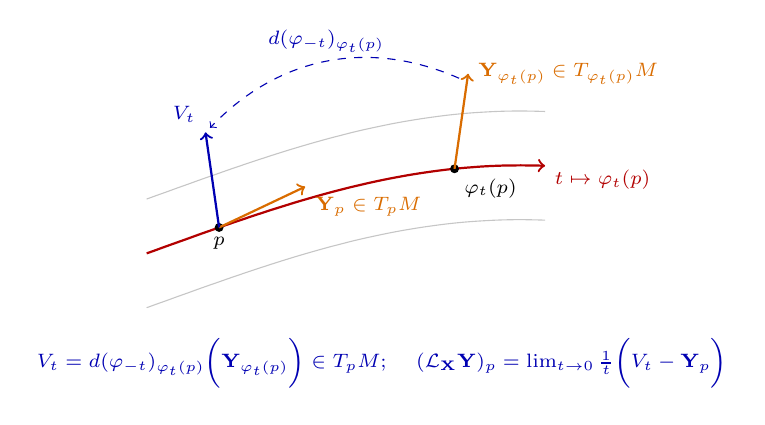
\begin{tikzpicture}[scale=1.15]
\draw[gray!45] plot[smooth] coordinates {(-2.400,-0.872) (-2.287,-0.831) (-2.174,-0.791) (-2.062,-0.750) (-1.949,-0.710) (-1.836,-0.669) (-1.723,-0.629) (-1.610,-0.590) (-1.497,-0.550) (-1.385,-0.512) (-1.272,-0.473) (-1.159,-0.436) (-1.046,-0.399) (-0.933,-0.363) (-0.821,-0.328) (-0.708,-0.294) (-0.595,-0.261) (-0.482,-0.229) (-0.369,-0.198) (-0.256,-0.169) (-0.144,-0.140) (-0.031,-0.113) (0.082,-0.088) (0.195,-0.064) (0.308,-0.041) (0.421,-0.020) (0.533,-0.001) (0.646,0.017) (0.759,0.033) (0.872,0.048) (0.985,0.061) (1.097,0.072) (1.210,0.081) (1.323,0.088) (1.436,0.094) (1.549,0.098) (1.662,0.100) (1.774,0.100) (1.887,0.098) (2.000,0.095)};
\draw[gray!45] plot[smooth] coordinates {(-2.400,0.328) (-2.287,0.369) (-2.174,0.409) (-2.062,0.450) (-1.949,0.490) (-1.836,0.531) (-1.723,0.571) (-1.610,0.610) (-1.497,0.650) (-1.385,0.688) (-1.272,0.727) (-1.159,0.764) (-1.046,0.801) (-0.933,0.837) (-0.821,0.872) (-0.708,0.906) (-0.595,0.939) (-0.482,0.971) (-0.369,1.002) (-0.256,1.031) (-0.144,1.060) (-0.031,1.087) (0.082,1.112) (0.195,1.136) (0.308,1.159) (0.421,1.180) (0.533,1.199) (0.646,1.217) (0.759,1.233) (0.872,1.248) (0.985,1.261) (1.097,1.272) (1.210,1.281) (1.323,1.288) (1.436,1.294) (1.549,1.298) (1.662,1.300) (1.774,1.300) (1.887,1.298) (2.000,1.295)};
\draw[thick, red!70!black, ->] plot[smooth] coordinates {(-2.400,-0.272) (-2.310,-0.240) (-2.220,-0.207) (-2.131,-0.175) (-2.041,-0.143) (-1.951,-0.111) (-1.861,-0.078) (-1.771,-0.046) (-1.682,-0.015) (-1.592,0.017) (-1.502,0.048) (-1.412,0.079) (-1.322,0.109) (-1.233,0.140) (-1.143,0.169) (-1.053,0.199) (-0.963,0.227) (-0.873,0.255) (-0.784,0.283) (-0.694,0.310) (-0.604,0.336) (-0.514,0.362) (-0.424,0.387) (-0.335,0.411) (-0.245,0.434) (-0.155,0.457) (-0.065,0.478) (0.024,0.499) (0.114,0.519) (0.204,0.538) (0.294,0.556) (0.384,0.573) (0.473,0.589) (0.563,0.604) (0.653,0.618) (0.743,0.631) (0.833,0.643) (0.922,0.654) (1.012,0.663) (1.102,0.672) (1.192,0.679) (1.282,0.686) (1.371,0.691) (1.461,0.695) (1.551,0.698) (1.641,0.699) (1.731,0.700) (1.820,0.699) (1.910,0.698) (2.000,0.695)};
\node[red!70!black, font=\scriptsize, anchor=west] at (2.00,0.54) {$t \mapsto \varphi_t(p)$};
\fill (-1.600,0.014) circle (1.4pt) node[below, font=\scriptsize] {$p$};
\fill (1.000,0.662) circle (1.4pt) node[below right, font=\scriptsize] {$\varphi_t(p)$};
\draw[->, thick, orange!85!black] (-1.600,0.014) -- ++(0.95,0.45) node[below right, font=\scriptsize] {$\mathbf{Y}_p \in T_pM$};
\draw[->, thick, orange!85!black] (1.000,0.662) -- ++(0.15,1.05) node[right, font=\scriptsize, align=center] {$\mathbf{Y}_{\varphi_t(p)} \in T_{\varphi_t(p)}M$};
\draw[->, thick, blue!70!black] (-1.600,0.014) -- ++(-0.15,1.05) node[above left, font=\scriptsize] {$V_t$};
\draw[->, blue!70!black, dashed] (1.050,1.662) to[bend right=35] node[above=2pt, font=\scriptsize, fill=white, inner sep=1pt] {$d(\varphi_{-t})_{\varphi_t(p)}$} (-1.700,1.114);
\node[font=\scriptsize, blue!70!black, anchor=north, align=center] at (0.2,-1.1) {$V_t = d(\varphi_{-t})_{\varphi_t(p)}\big(\mathbf{Y}_{\varphi_t(p)}\big) \in T_pM$; \quad $(\mathcal{L}_{\mathbf{X}}\mathbf{Y})_p = \lim_{t \to 0} \frac{1}{t}\big(V_t - \mathbf{Y}_p\big)$};
\end{tikzpicture}
